\documentclass[11pt,a4paper]{article}

\usepackage[margin=2.7cm]{geometry}
\usepackage[T1]{fontenc}
\usepackage{lmodern}
\usepackage{amsmath,amssymb,amsthm}
\usepackage{graphicx}
\usepackage{booktabs}
\usepackage{microtype}
\usepackage[dvipsnames]{xcolor}
\usepackage[colorlinks=true,linkcolor=MidnightBlue,citecolor=MidnightBlue,urlcolor=MidnightBlue]{hyperref}

\graphicspath{{figures/}}

\newtheorem{proposition}{Proposition}
\newtheorem{observation}{Observation}
\newtheorem{remark}{Remark}
\theoremstyle{definition}
\newtheorem{definition}{Definition}
\newtheorem{convention}{Convention}

\newcommand{\Etop}{E_{\mathrm{top}}}
\newcommand{\Emax}{E_{\mathrm{max}}}
\newcommand{\Ereach}{E_{\mathrm{reach}}}
\newcommand{\hPa}{\,\mathrm{hPa}}
\newcommand{\Jkg}{\,\mathrm{J\,kg^{-1}}}
\newcommand{\K}{\,\mathrm{K}}
\newcommand{\ms}{\,\mathrm{m\,s^{-1}}}

\title{An artificial discontinuity in the tcpyPI pressure solver:\\
a mathematical anatomy of issue \#77}
\author{Analysis prepared from the \texttt{tcpyPI} source, the PR~\#77
regression data, and the 2024 sample benchmark}
\date{July 12, 2026}

\begin{document}
\maketitle

\begin{abstract}
\noindent
The potential-intensity solver in \texttt{tcpyPI} (a Python port of Emanuel's
\texttt{pcmin}) computes a central pressure by fixed-point iteration
$x_{n+1}=g(x_n)$ and, for the sounding of PR~\#77 --- Hurricane Francine's
pre-landfall environment in a counterfactual-SST sensitivity member --- locks
into a bit-exact period-2 cycle instead of converging.  We show that the map
$g$ is \emph{discontinuous}, that its only diagonal crossing falls inside a
downward jump of $0.84\hPa$ at $x_d\simeq950.8289947515\hPa$ --- so
\emph{no fixed point exists} --- and we locate the source precisely: a
discontinuous \emph{selection rule} inside the CAPE routine (``integrate the
signed buoyancy up to the topmost grid level where buoyancy is positive, then
clamp at zero'').  A one-bit sign decision at the $350\hPa$ level, taken on a
marginal buoyancy feature worth $O(10^{-2})\Jkg$, toggles the inclusion of
$287\Jkg$ of negative area and moves the eyewall CAPE between $0$ and
$224\Jkg$.  Smooth toy models prove the pathology is a property of the
selection functional, not of grid resolution, quadrature, or interpolation,
and separate it from the \emph{genuine} discontinuities of the underlying
variational problem (the maximizer, by Berge's maximum theorem; the reachable
energy at barrier tangencies).  The mechanism is generic --- $20\%$ of
sampled real columns carry at least one jump of $g$ --- while the fatal
alignment with the diagonal is rare ($\sim0.04\K$ of SST for this column),
which is exactly why parameter sweeps find it.  The repair is to define CAPE
as the \emph{value function} $\max_q W(q)$ of the running signed work --- the
convention that also matches the physics of forced eyewall ascent --- and to
solve the pressure equation with a residual-checked bracketed method.  On
both known failing soundings this converges immediately (exact roots
$950.3137$ and $960.7687\hPa$); on a 7{,}093-column benchmark it changes no
convergence flags and leaves $98.1\%$ of intensities within $0.1\ms$, and it
renders the period-2 ``rescue'' logic dead code.
\end{abstract}

\tableofcontents

%======================================================================
\section{Conclusions first}\label{sec:conclusions}
%======================================================================

\begin{enumerate}
\item \textbf{The failure is exactly reproducible and is not slow
convergence.}  The iteration alternates bit-exactly between
$A=950.653345443832$ and $B=951.279007983853\hPa$; the separation
($0.626\hPa$) exceeds the $0.5\hPa$ stopping tolerance forever.  Raising the
iteration cap cannot help.
\item \textbf{No fixed point exists.}  The map $g$ jumps downward by
$0.837\hPa$ at $x_d\simeq950.8289947515\hPa$; the residual $g(x)-x$ passes
from $+0.507$ to $-0.331\hPa$ across the jump without taking the value zero.
A sign-change search reports $x_d$, but that is the location of a jump, not
a root.
\item \textbf{The cause is one discontinuous selection.}  In \texttt{cape()},
the level of neutral buoyancy is taken to be the \emph{highest sampled level
with positive buoyancy}.  For the eyewall parcel this one-bit decision moves
the terminal level between $750$ and $350\hPa$, dragging $287\Jkg$ of
intervening negative area into a signed integral that is then clamped at
zero: eyewall CAPE flips between $224.23\Jkg$ and $0$.  The saturated CAPE,
outflow temperature, and outflow level are smooth there --- the discontinuity
is not in the outflow calculation and not a quadrature error.
\item \textbf{The same mechanism explains the historical 1995 failure}
(cycle $961.017\leftrightarrow961.671\hPa$, triggered by the $400\hPa$
sample; eyewall CAPE flips $0\leftrightarrow203\Jkg$), while an adjacent-day
control column has an ordinary continuous root and converges.
\item \textbf{The repair is one changed selection plus one changed solver.}
Define CAPE as the maximum of the \emph{same} running signed work over
candidate terminal levels ($\Emax=\max_qW(q)$; Berge's maximum theorem makes
the value continuous even when the maximizing level jumps), and solve
$g(x)=x$ with residual-checked bracketing.  Negative-buoyancy layers still
count against the work; nothing is skipped or free.  Exact corrected results:
$x_*=950.3136889226\hPa$, $V_{\max}=83.9065\ms$, $P_{\min}=920.7517\hPa$ for
\#77, and $x_*=960.7687\hPa$, $V_{\max}=74.4149\ms$ for the 1995 case, each
confirmed by two independent implementations of the map.  The upstream
period-2 ``rescue''
(midpoint collapse) is then dead code; its midpoint $\approx950.966\hPa$ was
never a root of the stated equation.
\end{enumerate}

%======================================================================
\section{The computation, stripped of meteorology}
%======================================================================

\noindent\fbox{\begin{minipage}{0.965\linewidth}
\small
\textbf{Glossary for the mathematician}\par\smallskip
\textbf{Pressure as vertical coordinate.}  In atmospheric science the
vertical coordinate is pressure $p$, measured in hectopascals (hPa); $p$
decreases monotonically with altitude, from $\sim 1000\hPa$ at sea level to
$0$ at the top of the atmosphere.  ``Above'' means ``smaller $p$''.  Data
comes on a finite grid of \emph{pressure levels} $p_0 > p_1 > \dots > p_N$.

\textbf{Parcel.}  An idealized blob of air lifted adiabatically from a
starting level through the environment.  Its temperature along the ascent is
determined by thermodynamics (conservation of entropy), \emph{not} by the
environment; the environment only enters through comparison.

\textbf{Buoyancy.}  $b(p)$ = (density temperature of the parcel at level $p$)
$-$ (density temperature of the environment at $p$), in Kelvin.  Positive
$b$ pushes the parcel up.  Density temperature is a smooth algebraic function
of temperature, moisture and pressure.

\textbf{CAPE} (convective available potential energy, $\Jkg$): the work the
buoyancy force can do on the parcel, an integral of $b$ described below.

\textbf{LNB} (level of neutral buoyancy): the level where an ascending
parcel's buoyancy returns to zero --- where it ``detrains'' (exits).  The
temperature there, the \emph{outflow temperature} $T_O$, sets the Carnot
efficiency of the storm-as-heat-engine.

\textbf{SST}: sea-surface temperature.  \textbf{MSL}: sea-level pressure far
from the storm.
\end{minipage}}

\subsection{The work integral and the CAPE conventions}

Fix a column: levels $p_0>\dots>p_N$ (the code retains levels with
$p_j>50\hPa$; $N+1=28$ for the soundings here), environmental temperatures
$T_j$ and moisture $r_j$.  For a parcel specified by its starting pressure,
temperature and moisture, thermodynamics produces a buoyancy value $b_j$ at
every level: below its condensation level by an explicit smooth formula,
above it by inverting a smooth, strictly monotone entropy relation (a
guarded Newton iteration in the code).

\begin{observation}\label{obs:cont}
Each $b_j$ is a continuous --- indeed, away from one benign switch,
real-analytic --- function of the parcel parameters.  (The Newton stopping
tolerance of $10^{-3}\K$ and a formula switch at the condensation level
introduce micro-jumps of order $\lesssim10^{-3}\K$ in $b_j$; these propagate
to $\lesssim10^{-2}\hPa$ in the pressure map, $50\times$ below the solver
tolerance, and are accounted for separately in \S\ref{sec:micro}.)
\end{observation}

Define the \emph{running work integral} from the parcel's starting pressure
$q_0$ up to a trial ``outflow'' pressure $q\le q_0$:
\begin{equation}\label{eq:W}
W(q) \;=\; R_d \int_{q}^{q_0} b(p)\, \mathrm{d}\ln p ,
\end{equation}
where $R_d=287$ in SI units and $b(p)$ is the piecewise-linear interpolant of
the $b_j$.  The code evaluates \eqref{eq:W} by the trapezoid rule
$R_d(b_j+b_{j-1})(p_{j-1}-p_j)/(p_{j-1}+p_j)$ on grid intervals, plus a
partial term up to an interpolated zero of $b$ at the top --- i.e., exactly
the integral of the piecewise-linear reconstruction, with the terminal point
located \emph{sub-grid} by linear interpolation.  $W$ is a $C^1$-in-$q$,
piecewise-quadratic function whose critical points are the zeros of $b$:
local maxima at down-crossings ($b:+\to-$, candidate LNBs) and local minima
at up-crossings.  Figure~\ref{fig:anatomy} shows the generic anatomy: one
positive region of $b$, one hump of $W$, an unambiguous LNB at the argmax.

\begin{figure}[tb]
\centering
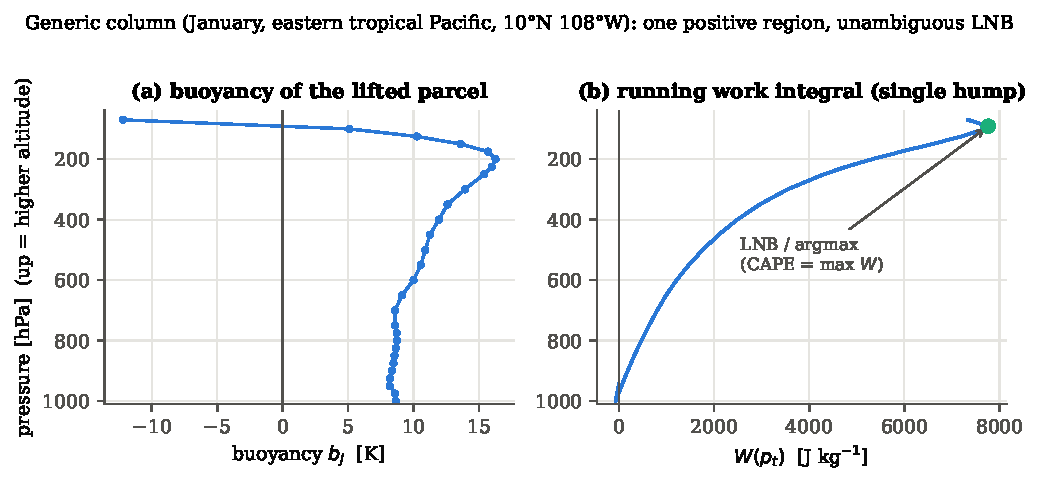
\includegraphics[width=0.86\linewidth]{fig_healthy_anatomy.pdf}
\caption{A generic strong-PI column (September, Caribbean; the saturated
parcel of \S\ref{sec:map}).  (a)~Buoyancy of the lifted parcel at the 28
retained grid levels.  (b)~The running work integral $W(q)$: a single
dominant hump; CAPE is its maximum, attained at the LNB.  For such profiles
every convention below coincides.}
\label{fig:anatomy}
\end{figure}

\begin{remark}[the two negative tails of $W$]\label{rem:tails}
In the $W$ figures the curve dips negative at \emph{both} ends, for
different reasons.  Above the LNB, $b<0$ and $W$ falls away from its
maximum --- mildly at first, then steeply in the stratosphere (to
$\approx-8000\Jkg$ by $70\hPa$ in the \#77 sounding; the figures clip this)
--- which is exactly what makes the LNB the argmax.  Near $1000\hPa$ the
negativity is bookkeeping, not ascent physics: $W$ is anchored at the
parcel's launch pressure $q_0=\min(x,1000)$, which for the storm-core
parcels lies \emph{above} the lowest data level because the trial central
pressure $x$ is below $1000\hPa$.  For $q>q_0$ (below the launch point)
$W(q)=-R_d\int_q^{q_0}b\,\mathrm d\ln p<0$ when the parcel is buoyant at the
bottom: displacing it downward costs work.  The code carries this segment as
a signed ``partial area between the parcel pressure and the lowest level''
correction (present identically in \texttt{pcmin.m}); the parcel never
visits it.  The anchor itself, $W(q_0)=0$, is a candidate terminal point ---
which is why $\Emax\ge0$ below holds with no clamp despite both tails.
\end{remark}

Turning $W$ into a single number requires choosing a terminal point, and
here conventions diverge.  Three natural choices:

\begin{convention}[value function]\label{conv:max}
$\displaystyle \Emax=\max_{q\in[p_N,\,q_0]} W(q)$, the value of the
parametric maximization; the LNB is the argmax.  Since $q=q_0$ is a
candidate with $W(q_0)=0$, automatically $\Emax\ge0$; no clamping is needed.
\end{convention}

\begin{convention}[ballistic / reachable]\label{conv:reach}
$\Ereach=\max\{W(q): q \text{ in the connected component of } \{W>0\}
\text{ containing } q_0\}$.  A parcel starting \emph{at rest} converts work
to kinetic energy and stalls where $W$ first returns to zero; $\Ereach$ is
the best energy among levels such a parcel can reach unaided.
\end{convention}

\begin{convention}[topmost-positive-level --- the code's rule]\label{conv:top}
Let $\mathrm{INB}=\max\{\,j : b_j>0\,\}$ (a \emph{grid} index).  Then
\[
\Etop=\max\Bigl(\,\text{signed integral up to level } \mathrm{INB}
\text{ plus the partial area up to the interpolated zero above it},\ 0\Bigr),
\]
where the outer $\max(\,\cdot\,,0)$ is the code's clamp of a possibly
negative signed integral to zero --- this clamp \emph{is} reachable here,
and is half of the issue-77 mechanism.
Equivalently: $\Etop=\max\bigl(W(z_{\mathrm{top}}),\,0\bigr)$ where
$z_{\mathrm{top}}$ is the topmost down-crossing of the piecewise-linear $b$
(or the profile top if $b_N>0$).
\end{convention}

Pointwise, $\Etop \le \Emax$ and $\Ereach\le\Emax$:
Convention~\ref{conv:top} evaluates $W$ at one particular candidate,
Convention~\ref{conv:max} at the best one.  For a single-hump $W$ --- the
overwhelmingly common case --- all three agree exactly.

\paragraph{Which convention does the physics of PI want?}
The word ``CAPE'' is misleading here.  In an ordinary sounding it is read as
kinetic energy available to a freely rising parcel, for which the ballistic
Convention~\ref{conv:reach} is the natural semantics.  The PI quantity is
instead \emph{hurricane CAPE}: in the Bister--Emanuel derivation the CAPE
difference is an alternative expression for the thermodynamic work around
the idealized storm cycle \cite{bisteremanuel2002,gilford2021}, and eyewall
ascent in a mature vortex is driven primarily by frictional convergence ---
organized, forced, predominantly hydrostatic --- not by a parcel coasting on
its own buoyancy \cite{garner2015}.  An intervening negatively buoyant layer
must still be \emph{charged against the work} (it reduces $W$), but it is
not a hard reachability barrier for the forced secondary circulation.  That
is precisely Convention~\ref{conv:max}: every layer costs what it costs,
and the outflow level is the one maximizing extractable work.  This
distinction drives the recommendation in \S\ref{sec:fix}.

\subsection{The fixed-point map}\label{sec:map}

The solver seeks the storm's central pressure $x$ (hPa) at the radius of
maximum winds.  Given a trial $x$, it computes three CAPE values with the
environment held fixed: $E_A$ (an $x$-independent ambient surface parcel),
$E_M(x)$ (the ambient surface parcel displaced to pressure $x$, which
enriches its moisture --- the ``eyewall parcel''), and $E_{MS}(x)$ (a parcel
saturated at the SST at pressure $x$ --- the storm-core parcel, whose LNB
also furnishes the outflow temperature $T_O(x)$).  These combine into
\begin{equation}\label{eq:g}
g(x) \;=\; \mathrm{MSL}\cdot
\exp\!\Bigl(-\,\mathrm{CAT}(x)\,/\,\bigl(R_d\,\overline{T}_v(x)\bigr)\Bigr),
\qquad
\mathrm{CAT}(x)=\max\Bigl((E_M{-}E_A)+\tfrac12\,\kappa\,
\tfrac{\mathrm{SST}}{T_O}\,(E_{MS}{-}E_M),\ 0\Bigr),
\end{equation}
with $\kappa=C_k/C_D=0.9$ and $\overline{T}_v$ a smooth positive function of
$x$.  The released code runs Picard iteration $x_{n+1}=g(x_n)$ from
$x_0=970$, stopping when consecutive iterates satisfy
$|x_{n+1}-x_{n}|\le 0.5\hPa$, capped at 200 steps.  (A two-back comparison
$|x_{n+1}-x_{n-1}|$ appears only in the recently added cycle-detection
patch, not in the stopping rule.)  All CAPE evaluations use
Convention~\ref{conv:top}.  Note that even for continuous $g$, Picard
iteration requires local contractivity $|g'(x_*)|<1$; existence of a fixed
point alone is not enough --- and for discontinuous $g$, neither existence
nor convergence is available.

Away from the pathologies below, $g$ is a mild contraction: on the failing
sounding its slope off the jump is $0.34$--$0.46$, and generic columns
converge geometrically (Fig.~\ref{fig:healthymap}).

\begin{figure}[tb]
\centering
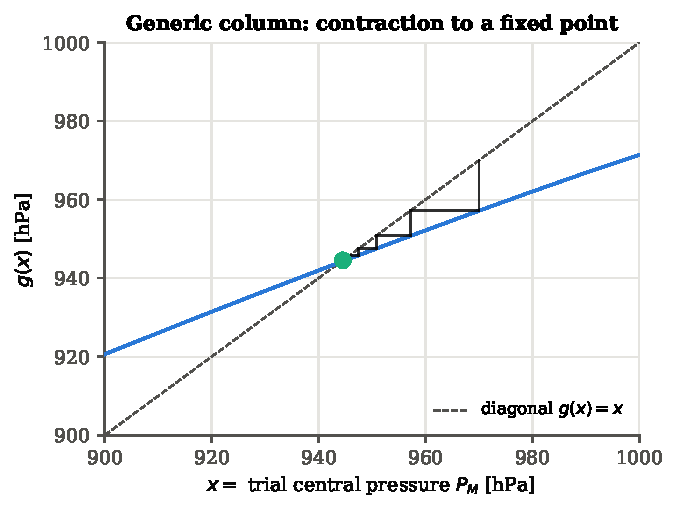
\includegraphics[width=0.5\linewidth]{fig_healthy_map.pdf}
\caption{The map $g$ for the generic column of Fig.~\ref{fig:anatomy}, with
the cobweb of the iteration from $x_0=970$: contraction to a fixed point at
$861.8\hPa$.}
\label{fig:healthymap}
\end{figure}

%======================================================================
\section{A smooth toy model: what is genuinely discontinuous}
\label{sec:toy}
%======================================================================

Everything essential can be exhibited with $C^\infty$ data, which settles at
the outset that grid resolution, quadrature order, and interpolation
smoothness are \emph{not} the cause (a claim tested directly on the real
sounding in \S\ref{sec:notcause}).  Take a smooth family of buoyancy
profiles on a height coordinate $t$,
\begin{equation}\label{eq:toy}
b(t)\;=\;\underbrace{0.6\,e^{-\left(\frac{t-0.22}{0.10}\right)^2}}_{\text{main
convective cell}}\;-\;\underbrace{\delta\,
e^{-\left(\frac{t-0.5}{0.12}\right)^2}}_{\text{stable ``valley''}}\;+\;
\underbrace{\varepsilon\,
e^{-\left(\frac{t-0.8}{0.06}\right)^2}}_{\text{upper feature}},
\end{equation}
with $W(t)=\int_0^t b$, and evaluate the three conventions along two sweeps
(Fig.~\ref{fig:toy}).

\begin{figure}[tb]
\centering
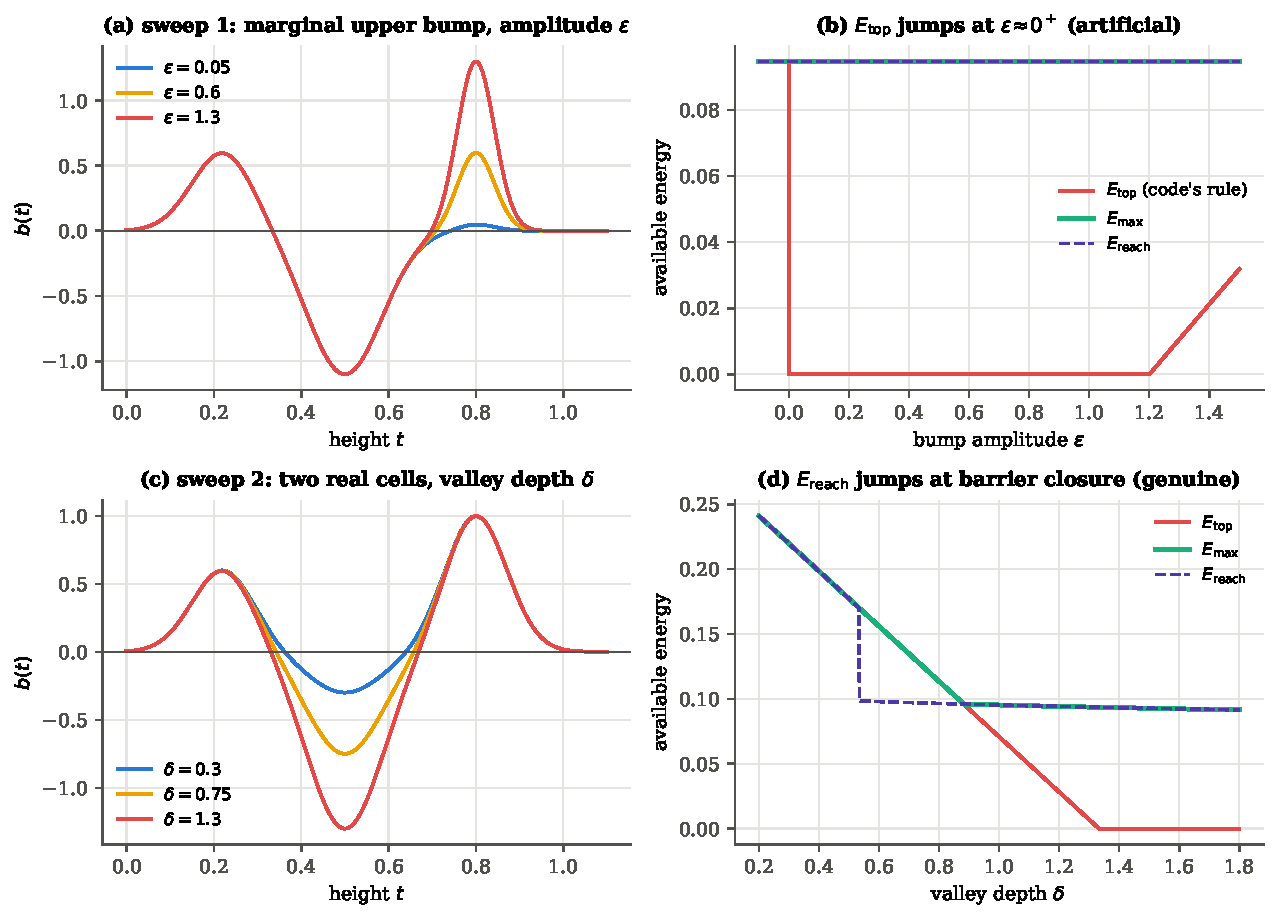
\includegraphics[width=0.98\linewidth]{fig_toy.pdf}
\caption{The smooth toy model \eqref{eq:toy}.
\textbf{Sweep 1} (top row; $\delta=1.1$ fixed): the amplitude $\varepsilon$ of
a \emph{marginal} upper bump crosses zero.  $\Etop$ jumps from $0.095$ to $0$
at $\varepsilon=0^+$: the instant the bump's peak becomes positive, the
topmost zero of $b$ teleports above it and the terminal value
$W\approx-0.13<0$ is clamped to $0$.  $\Emax$ and $\Ereach$ do not react at
all --- the bump is dominated \emph{and} unreachable.  This is the issue-77
mechanism in pure form.
\textbf{Sweep 2} (bottom row; two genuinely competing cells, valley depth
$\delta$ varies): $\Emax$ is continuous with a kink where the argmax
exchanges humps ($\delta=0.881$), while $\Ereach$ has a \emph{genuine}
downward jump at $\delta=0.534$, where the energy barrier closes and the
upper cell becomes ballistically unreachable.}
\label{fig:toy}
\end{figure}

The toy isolates three distinct behaviors:

\begin{enumerate}
\item \textbf{$\Emax$ is continuous, always} --- Berge's maximum theorem in
its simplest form: $W(\cdot;\lambda)$ is a jointly continuous family over a
fixed compact interval, so $\lambda\mapsto\max_q W(q;\lambda)$ is
continuous \emph{even where the argmax jumps}.  The argmax correspondence is
only upper hemicontinuous: at a dominance exchange the maximizer teleports
(by $455\hPa$ in the real-data example of \S\ref{sec:physical}), but the
value passes through with a kink, not a jump.
\item \textbf{$\Ereach$ can jump for real physical reasons}, but only at a
codimension-one tangency: the local minimum of $W$ in the valley touches
zero, the set $\{W>0\}$ changes topology, and the reachable energy jumps.
A bona-fide first-order transition --- but of the \emph{free-convection}
problem, which is not the PI problem (\S\ref{sec:physical}).
\item \textbf{$\Etop$ jumps at events with no physical content}: the sign of
$b$ at its topmost zero is toggled by an $O(\varepsilon)$ feature carrying
$O(\varepsilon)$ energy, dominated by orders of magnitude, and (in sweep 1)
sitting behind a closed barrier.  The discontinuity locus of the
``topmost positive point'' selector strictly contains the physical loci of
items 1--2 and is enormously larger.  The same holds for smooth fields in
general: an upper positive pocket is born at a fold ($b=0$, $\partial_t b=0$
simultaneously), and the uppermost-root diagnostic jumps there even though
$b$ is $C^\infty$ and the value function is not affected unless the new
pocket actually dominates.
\end{enumerate}

\subsection{Why the symptom is a bit-exact 2-cycle}

Insert a downward jump into an otherwise flat contraction so that the gap
straddles the diagonal: $g(x)-x>0$ on the left branch, $<0$ on the right.
No fixed point exists, every orbit must cross the jump forever, and because
$g$ is nearly constant on each side (slope $\ll1$), the branch values
$g(A)\approx B$ and $g(B)\approx A$ form a \emph{superattracting} 2-cycle:
$g\circ g$ contracts strongly onto each branch point, so the alternation
converges bitwise (Fig.~\ref{fig:toymap}).  The observed 16-digit lock is
the canonical dynamics of a gap-straddling contraction --- an attracting
border-collision cycle, not a curiosity of the sounding.

\begin{figure}[tb]
\centering
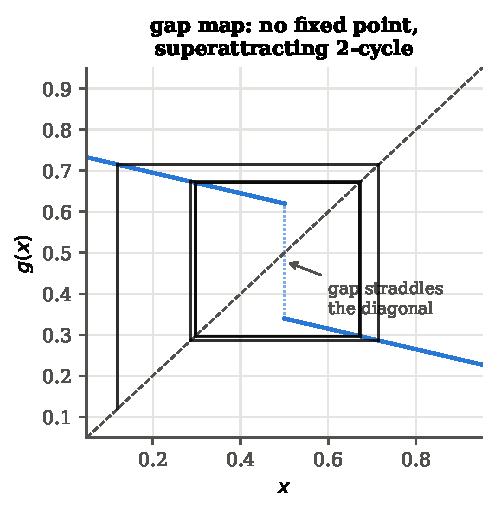
\includegraphics[width=0.4\linewidth]{fig_toymap.pdf}
\caption{Abstract gap map: piecewise-linear contraction (slope $0.25$) with a
downward jump straddling the diagonal.  Orbits fall into the unique 2-cycle
$\{g(B),g(A)\}$; the cycle is superattracting because $|g'(A)g'(B)|\ll1$.}
\label{fig:toymap}
\end{figure}

%======================================================================
\section{The failure in the wild: Hurricane Francine, issue \#77}
\label{sec:pr77}
%======================================================================

\subsection{Provenance}

The failing sounding is the environment of an \emph{actual tropical
cyclone}.  PR~\#77 records $28.6^{\circ}$N, $92.1^{\circ}$W at 18~UTC on
September 11, 2024 --- and the National Hurricane Center best track places
Hurricane Francine at exactly that position and time, at 80~kt a few hours
before its Louisiana landfall \cite{francine,pr77}.  The thermodynamic
column is a \emph{counterfactual-climate sensitivity member} associated with
the storm (SST perturbed by $-1.6\K$, mapped to a 1994/day-263 reference),
not an in-situ measurement --- a distinction that matters physically but not
to the numerical diagnosis.  The failure thus arises while asking the
operational question this code exists to answer: \emph{how strong could this
storm have been in a cooler climate?}  For that member the solver returns
``missing''.  Column parameters: SST $=28.203^{\circ}$C, MSL
$=1014.97\hPa$, 37 levels (28 retained).

\subsection{The map has no fixed point}

Scanning $g$ at $0.002\hPa$ resolution over $[946,958]$
(Fig.~\ref{fig:pr77map}) yields:

\begin{observation}\label{obs:pr77}
On $[946,958]$ the map $g$ has exactly one discontinuity, a downward jump of
$0.837\hPa$ at $x_d\simeq950.8289947515\hPa$.  The residual $F(x)=g(x)-x$
satisfies $F>0$ for $x<x_d$ and $F<0$ for $x>x_d$ (Fig.~\ref{fig:capem}b):
the only sign change occurs across the jump, so $g$ has no fixed point.
Away from $x_d$, $g$ is smooth with slope $0.34$--$0.46$.  The iterates
converge to the 2-cycle $\{A,B\}$ straddling $x_d$.
\end{observation}

\begin{figure}[tb]
\centering
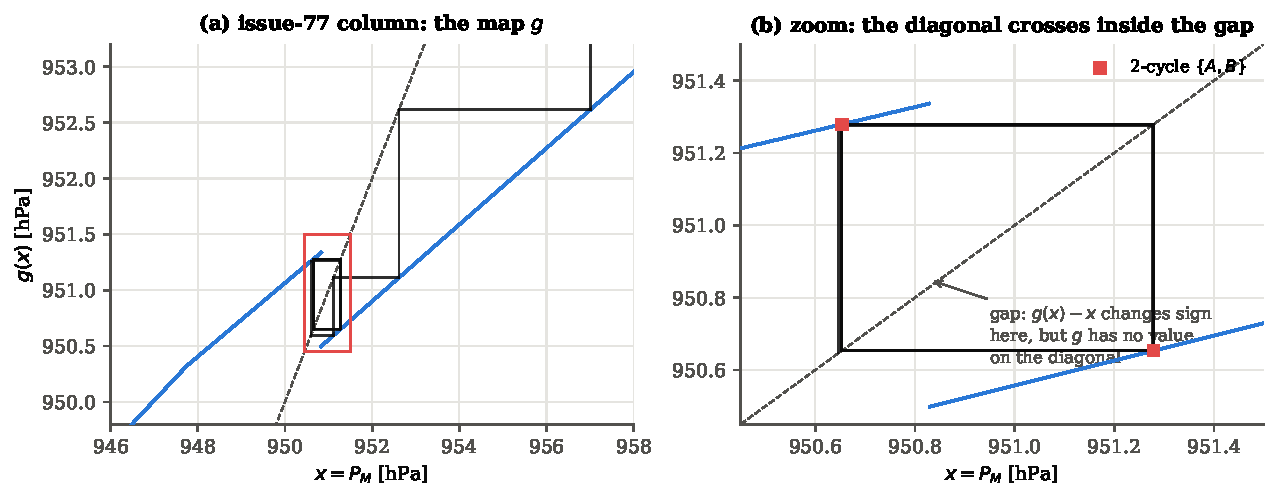
\includegraphics[width=0.98\linewidth]{fig_pr77_map.pdf}
\caption{The issue-77 map (Hurricane Francine's environment, $-1.6\K$
counterfactual).  (a)~$g$ on $[946,958]$ with the iteration cobweb from
$x_0=970$; the red box marks the zoom.  (b)~Zoom: two smooth branches
separated by a $0.837\hPa$ gap; the diagonal passes through the gap; the
iteration locks into the bit-exact 2-cycle (red squares).}
\label{fig:pr77map}
\end{figure}

\subsection{One-sided anatomy of the jump}

Evaluating all internal quantities $10^{-9}\hPa$ on either side of $x_d$
isolates the discontinuous term:

\begin{center}
\small
\begin{tabular}{lrr}
\toprule
quantity & $x_d-10^{-9}$ & $x_d+10^{-9}$ \\
\midrule
buoyancy sample at $350\hPa$ (K) & $+7.58\times10^{-11}$ & $-7.99\times10^{-11}$ \\
highest positive index & 18 ($350\hPa$) & 10 ($750\hPa$) \\
diagnosed LNB (hPa) & $350.0000$ & $741.4664$ \\
eyewall CAPE $E_M$ ($\Jkg$) & $0$ & $224.23146$ \\
saturated CAPE $E_{MS}$ ($\Jkg$) & $8565.00966$ & $8565.00966$ \\
saturated outflow $T_O$ (K) & $206.1096884$ & $206.1096884$ \\
$g(x)$ (hPa) & $951.3363394$ & $950.4982353$ \\
$F(x)=g(x)-x$ (hPa) & $+0.5073447$ & $-0.3307594$ \\
\bottomrule
\end{tabular}
\end{center}

\noindent
The saturated terms --- and hence the outflow temperature entering
\eqref{eq:g} --- are smooth; the discontinuity is entirely in the eyewall
parcel's $E_M$, through the selector of Convention~\ref{conv:top}.
(The $10^{-11}\K$ values demonstrate the one-sided limit; they are not the
amplitude of the atmospheric feature.  At the two cycle phases the $350\hPa$
buoyancy is $+0.0137$ and $-0.0350\K$: marginal and energetically
negligible, but not floating-point noise.)

Figure~\ref{fig:mech} shows the geometry.  The eyewall parcel's buoyancy has
a healthy positive region below $750\hPa$ (the main hump of $W$, worth
$\approx222$--$224\Jkg$ depending on the trial pressure), a deep negative
valley from $750$ to $400\hPa$ ($-287\Jkg$), and the marginal excursion at
the $350\hPa$ node.  When that node's sign flickers positive, the selector
teleports its terminal point from $\approx745$ to $350\hPa$, the signed
integral becomes $226.6+0.01-287.5=-60.9\Jkg$, and the final clamp
$\max(\,\cdot\,,0)$ maps it to $0$.  Composing the three steps,
\[
b\;\longmapsto\;\mathrm{INB}=\max\{j: b_j>0\}
\;\longmapsto\; W(z_{\mathrm{top}})
\;\longmapsto\; \max(\,\cdot\,,0),
\]
the first arrow is the discontinuous one; the clamp then pins one side to
the constant $0$, maximizing the jump.  Note also (Fig.~\ref{fig:mech}b)
that $W(350\hPa)=-61\Jkg<0$: even a ballistic parcel could never reach the
level whose sign decides between $224$ and $0$ --- it would stall inside the
valley.  Under \emph{every} available physical semantics ($\Emax$,
$\Ereach$) the answer on both sides of the flicker is the same
$\approx222\Jkg$.

\begin{figure}[tb]
\centering
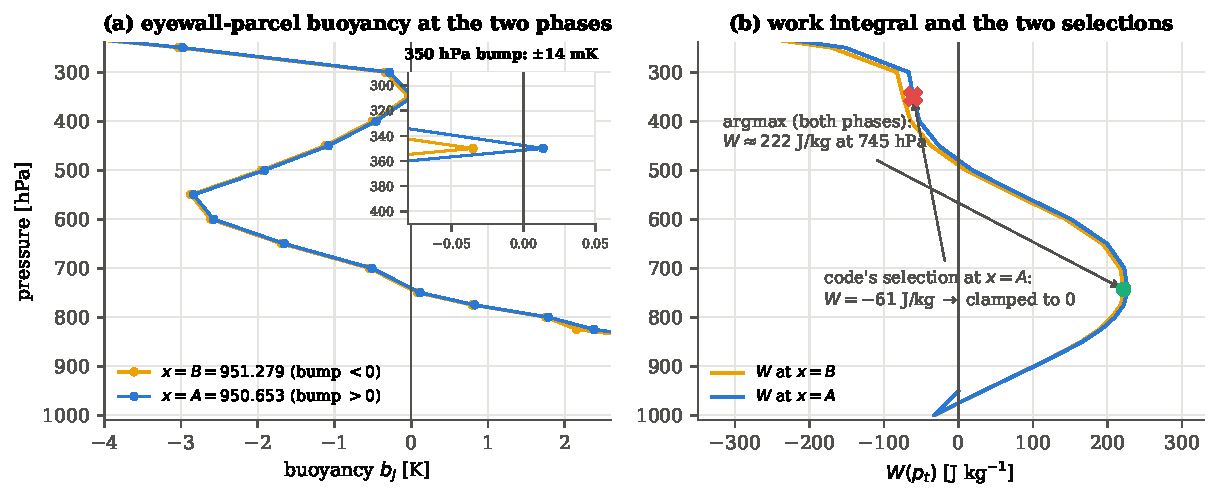
\includegraphics[width=0.98\linewidth]{fig_pr77_mechanism.pdf}
\caption{The issue-77 mechanism.  (a)~Eyewall-parcel buoyancy at the two
cycle phases (curves nearly coincide); inset: the marginal excursion at
$350\hPa$ whose sign differs between phases by $\pm14$~mK.  (b)~The
corresponding work integrals: the argmax ($222\Jkg$ at $745\hPa$, green) is
identical in both phases; the code's terminal point at phase $A$ (red cross)
sits at $350\hPa$ where $W=-61\Jkg$, clamped to $0$.}
\label{fig:mech}
\end{figure}

\begin{figure}[tb]
\centering
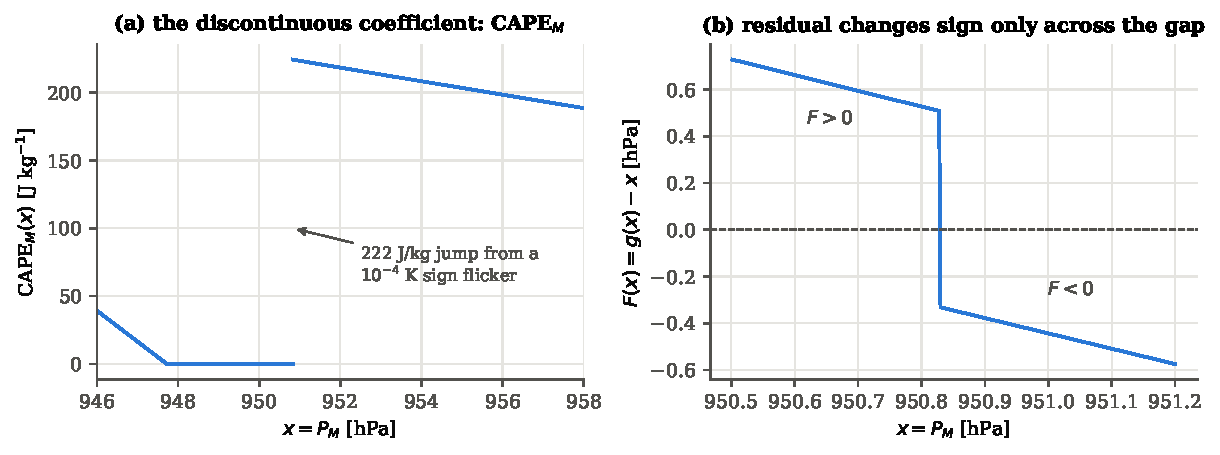
\includegraphics[width=0.98\linewidth]{fig_pr77_capem.pdf}
\caption{(a)~$E_M$ as a function of the trial pressure $x$: piecewise smooth
with the cliff at $x_d$ (the structure at $x<948$ is a second, harmless
flicker of the same kind).  (b)~The residual $F=g-x$ near $x_d$: the only
sign change is across the gap; no root exists.}
\label{fig:capem}
\end{figure}

\subsection{The second instance, and the control}

The 1995 sounding of the repository's regression tests fails by the
identical geometry (Fig.~\ref{fig:1995}): its $400\hPa$ sample flickers,
$E_M$ flips $0\leftrightarrow203.05\Jkg$, the residual jumps
$+0.615\to-0.225\hPa$, and the iteration cycles at
$961.017\leftrightarrow961.671\hPa$.  An adjacent-day
control profile has an ordinary continuous crossing and converges --- the
failure is a property of marginal columns, not of the data source.  Both
failing columns are \emph{marginal} in the precise sense that the ambient
CAPE $E_A$ is tiny ($1.19\Jkg$ for \#77; exactly $0$ for both 1995 profiles
under the released quadrature): selector topology matters most near such
boundaries, where the clamp is live and humps are shallow.

\begin{figure}[tb]
\centering
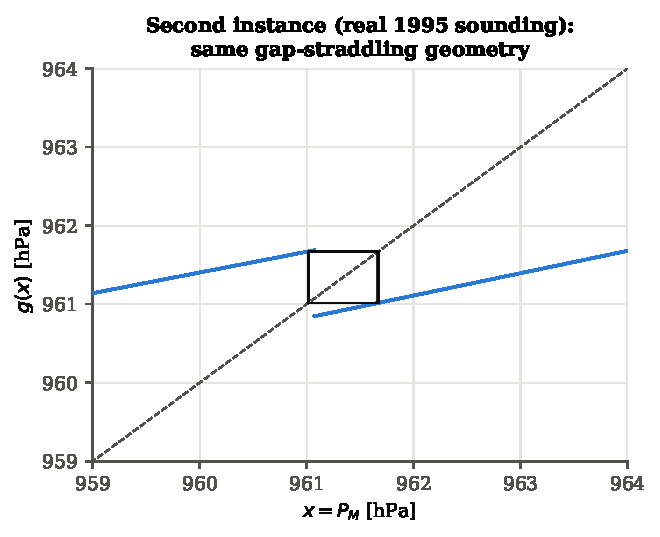
\includegraphics[width=0.48\linewidth]{fig_1995_map.pdf}
\caption{The second known failing sounding (real 1995 profile): the same
gap-straddling geometry and 2-cycle.}
\label{fig:1995}
\end{figure}

\subsection{Why the upstream ``rescue'' is not a solution}

A recent upstream patch detects the 2-cycle and collapses it to its
midpoint ($\approx950.966\hPa$ here), exiting through the normal
convergence path.  But the one-sided residuals at the jump are $+0.507$ and
$-0.331\hPa$: \emph{there is no root there to approximate}.  The midpoint is
a convention for returning a number, not a solution of $g(x)=x$; moreover
the thermodynamic fields ultimately reported are evaluated at one cycle
phase, an arbitrary parity-dependent choice worth $\sim1.2\ms$ in
$V_{\max}$.  Cycle detection remains useful as telemetry and as a guard
against burning 200 iterations, but it treats the symptom.  The disease is
the discontinuity.

%======================================================================
\section{What is generic, what is unusual}
\label{sec:generic}
%======================================================================

Two separate questions: how common are jumps of $g$, and how common is the
\emph{fatal configuration} (diagonal crossing inside a jump)?

We scanned $g$ at $0.1\hPa$ resolution over $x\in[900,1005]$ for 1{,}200
randomly sampled converging columns of the repository's 2024 North-Atlantic
sample (Fig.~\ref{fig:survey}a).  \textbf{Jumps are generic}: $239/1200$
columns ($20\%$) carry at least one jump, with sizes up to $\sim1\hPa$ ---
unsurprising, since the tropical upper troposphere hovers near moist
neutrality ($b\approx0$ over deep layers), so marginal sign flickers under
the $x$-dependent parcel moisture are everywhere.  \textbf{The fatal
configuration is rare}: in zero of the 1{,}200 columns does the diagonal
crossing fall inside a jump, consistent with the full 7{,}093-column sample
containing no convergence failures.

How close is ``close''?  Perturbing the Francine column's SST further
(Fig.~\ref{fig:survey}b), the no-fixed-point window is $\sim0.04\K$ wide out
of $6\K$ scanned.  This explains where the failure surfaced: an
SST-attribution sweep around a real storm samples SST densely and will
eventually land inside some column's window.  Single climatological runs
rarely hit it; parameter sweeps over live cases --- where a silently missing
value is most costly --- will.  The alignment is also less improbable than
it looks: the iteration actively ferries orbits from both sides back across
the jump, so once the crossing is inside the gap the cycle is
\emph{attracting}, and a jump elsewhere passes unnoticed (either it does not
straddle zero, or the induced cycle amplitude is below the $0.5\hPa$
tolerance and is silently accepted as convergence).

\begin{figure}[tb]
\centering
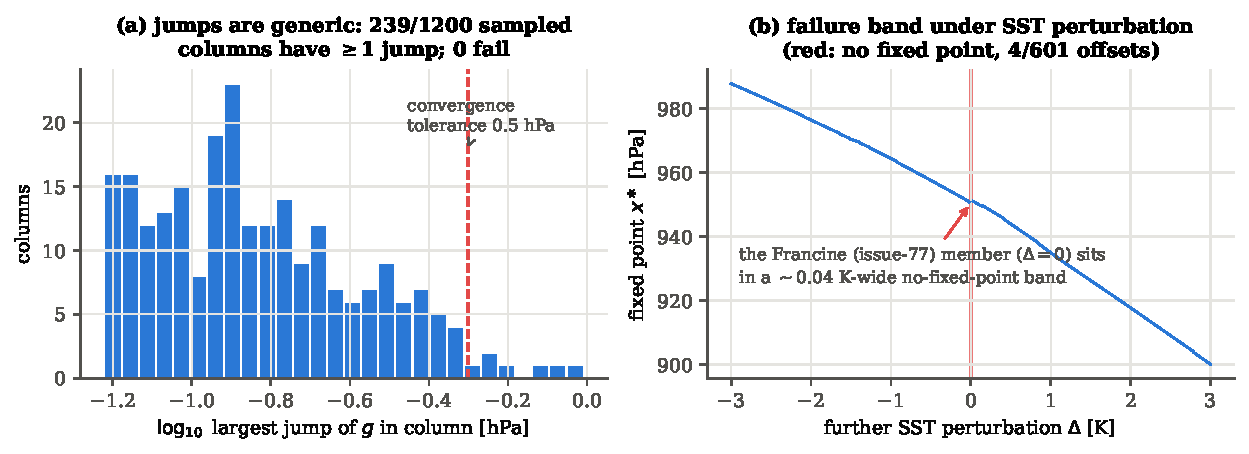
\includegraphics[width=0.98\linewidth]{fig_survey.pdf}
\caption{(a)~Largest jump of $g$ per column over 1{,}200 sampled real columns
(only the 239 with a detected jump shown).  Jumps are common; none coincides
with its column's diagonal crossing.  (b)~The Francine column under further
SST perturbation: the fixed point moves smoothly except in a $\sim0.04\K$
band (red) where it does not exist; the issue-77 member sits inside it.}
\label{fig:survey}
\end{figure}

%======================================================================
\section{To what extent is the discontinuity physical?}
\label{sec:physical}
%======================================================================

Argmax-type constructions \emph{do} have genuine discontinuities, and one
must not repair those away.  The precise accounting:

\paragraph{The maximizer may genuinely jump; the value may not.}
CAPE-as-energy is the \emph{value} of $\max_q W(q;\lambda)$; the LNB and
outflow temperature are the \emph{maximizer}.  By the maximum theorem the
value is continuous in the data; the maximizer is only upper hemicontinuous
and jumps at dominance exchanges.  Figure~\ref{fig:bergefig} shows this on a
real column: a $0.4\%$ moisture change teleports the argmax
$870\to410\to180\hPa$ while the value crosses each exchange with a kink.
Physically the maximizer's jump is a real bifurcation --- the preferred
detrainment layer switches --- and any code reporting $T_O$ must live with
it.  (In \eqref{eq:g}, $T_O$ comes from the \emph{saturated} parcel, whose
$W$ is single-humped with a $\sim40\times$ dominance margin for
storm-relevant SSTs, so this genuine discontinuity is dormant in practice;
see \S\ref{sec:micro}.)  The maximizing level is in any case metadata rather
than a prediction: where real eyewall air detrains depends on dynamics and
mixing absent from a reversible parcel calculation.

\begin{figure}[tb]
\centering
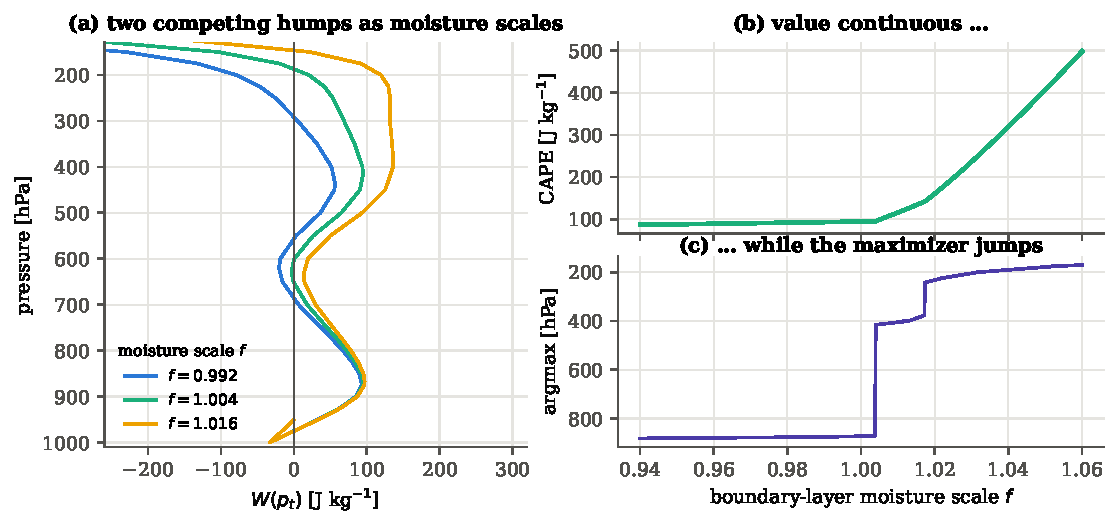
\includegraphics[width=0.98\linewidth]{fig_berge.pdf}
\caption{Berge's theorem on a real column (June, $28.5^{\circ}$C SST).
(a)~The eyewall-parcel work integral has two competing humps $450\hPa$
apart.  (b,c)~Sweeping boundary-layer moisture by $\pm6\%$: CAPE
$=\max_qW$ is continuous through both dominance exchanges (kinks), while
the argmax jumps.  Value and maximizer have different continuity classes;
only the maximizer's jumps are physical.}
\label{fig:bergefig}
\end{figure}

\paragraph{Reachable energy can genuinely jump --- in a different problem.}
Under ballistic semantics (Convention~\ref{conv:reach}) the value itself
jumps when an energy barrier closes at a tangency (toy sweep 2).  That is
legitimate physics --- of \emph{spontaneous free convection}: an isolated
parcel launched from rest does not teleport through a barrier.  It is not
the physics of hurricane PI, whose eyewall ascent is forced by the storm's
own frictionally convergent circulation \cite{garner2015,bisteremanuel2002}.
A reachability-restricted CAPE answers a different question and should at
most be a separately named diagnostic, never the PI default
(\S\ref{sec:fix}).

\paragraph{The code's discontinuity is neither of these.}
Convention~\ref{conv:top} jumps whenever the topmost sign of $b$ flickers
--- a strict superset of the physical loci above.  At the issue-77 event
specifically: the deciding feature carries $O(10^{-2})\Jkg$ against a
$224\Jkg$ decision (no energetic semantics); the selected terminal level has
$W=-61\Jkg$, unreachable even ballistically (no reachability semantics);
and both $\Emax$ and $\Ereach$ are constant through the event.  If the
``topmost level'' rule encodes an intention --- ``outflow happens at the
highest level convection can reach'' --- then $\Emax$'s argmax honors that
intention on every profile where the top level is attainable and worth
attaining; where the rules differ, $\Etop$ is charging the parcel an entry
fee for a room it never enters.

\begin{center}
\small
\begin{tabular}{@{}p{0.30\linewidth}p{0.24\linewidth}p{0.36\linewidth}@{}}
\toprule
feature & status & reason \\
\midrule
multiple buoyant layers & physical possibility & stratification can create
several neutral levels \\
birth of a remote positive pocket & genuine mathematics & a smooth field can
undergo a fold/tangency \\
maximizing LNB jumping & genuine (variational) & work maxima exchange
dominance; the common value stays continuous (Berge) \\
reachable energy jumping & genuine, wrong problem & barrier closure is
free-convection physics, not forced-ascent PI \\
uppermost-positive-node jumping & genuine mathematics, wrong value rule &
that node need not maximize work nor be reachable \\
$E_M$ jumping $0\leftrightarrow224\Jkg$ & artifact & selector $+$ signed
integration $+$ clamp amplify a one-bit sign \\
pressure two-cycle & solver artifact & a discontinuous map is iterated as
though contractive \\
\bottomrule
\end{tabular}
\end{center}

\subsection{What the cause is not}\label{sec:notcause}

Three natural alternative hypotheses were tested and refuted, and deserve
one paragraph so nobody re-litigates them.  \emph{Quadrature order}: the
trapezoid rule with sub-grid terminal crossings integrates the
piecewise-linear reconstruction exactly and handles simple crossings
continuously; the jump survives with the same quadrature under
Convention~\ref{conv:max}, and disappears with the same quadrature under a
changed \emph{selection} --- the quadrature is innocent.  \emph{Grid
resolution / interpolation smoothness}: rebuilding the Francine environment
with a $C^1$ monotone-cubic interpolant of $T,r$ in $\ln p$ resampled at
$5\hPa$ resolves the $350\hPa$ feature (it is real, and $4\times$ taller
than the coarse grid shows) and happens to converge --- but the map still
has an $0.83\hPa$ jump, merely relocated to $951.4\hPa$, off the diagonal
\emph{by luck}; the same resampling with linear interpolation leaves the
jump straddling the diagonal and still fails.  No reconstruction, of any
smoothness class, can remove the discontinuity of $\Etop$: \S\ref{sec:toy}
exhibits it for $C^\infty$ data.  \emph{Floating point}: the one-sided
$10^{-11}\K$ values are ordinary continuity of $b_{18}(x)$ through zero, not
roundoff; the feature itself is tens of millikelvin at the cycle phases.
Discretization's real role is secondary: it quantizes \emph{where} flickers
can fire (at nodes) and lends a $\sim100\hPa$-wide lever arm to a narrow
feature, but the selection rule decides \emph{that} they fire.

%======================================================================
\section{The repair}
\label{sec:fix}
%======================================================================

\subsection{Maximum-work CAPE: one changed selection}

Replace Convention~\ref{conv:top} by Convention~\ref{conv:max} in all three
CAPE evaluations of \eqref{eq:g}: accumulate the \emph{same} running signed
work $W$ over the \emph{same} piecewise-linear reconstruction with the
\emph{same} sub-grid crossing candidates, and take the maximum over
candidate terminal points instead of the value at the topmost crossing.
Return the argmax as the LNB (with an explicit tie rule).  No clamp is
needed.  Nothing is skipped and nothing is free: every negative-buoyancy
layer reduces $W$ along the way.  The change is one selection, not new
machinery --- and for single-hump profiles it reproduces the legacy value
exactly.

This is also the physically correct convention for PI
(\S\ref{sec:physical}): hurricane CAPE is thermodynamic work around a
forced cycle, so the outflow level is the one maximizing extractable work,
with traversal costs charged but no ballistic reachability requirement.
The ballistic (first-connected-lobe) rule was also implemented as a
proof-of-mechanism: it too removes the failures, but it answers the
free-convection question ---
and it perturbs the healthy control column by $1.2\hPa$ where max-work
moves it by $0.0035\hPa$.  Maximum signed work is the minimal-change,
correct-semantics repair.

\subsection{Existence, and solving for a root}

\begin{proposition}\label{prop:cont}
With $\Emax$ in place of $\Etop$ in all three CAPE evaluations, and modulo
the micro-jumps of \S\ref{sec:micro}, the map $g$ of \eqref{eq:g} is
continuous on $[400,\mathrm{MSL}]$ wherever the saturated parcel's argmax is
unique, and $g\le\mathrm{MSL}$ so that $F(x)=g(x)-x$ satisfies
$F(\mathrm{MSL})\le0$.  If in addition the column satisfies the
non-hypercane endpoint condition $g(400)>400$, then $F(400)>0$ and the
intermediate value theorem gives a fixed point in $(400,\mathrm{MSL}]$.
\end{proposition}

\begin{proof}[Proof sketch]
Each $b_j$ is continuous in $x$ (Observation~\ref{obs:cont}); $W$ is jointly
continuous on a compact set; $\Emax=\max_qW$ is continuous (maximum
theorem); $E_A$ is constant and $\overline T_v$ smooth and positive;
$T_O(x)$ is continuous wherever the saturated argmax is unique;
$\max(\,\cdot\,,0)$ and $\exp$ preserve continuity.  $\mathrm{CAT}\ge0$
gives $g\le\mathrm{MSL}$.
\end{proof}

Both hypotheses are explicit for a reason.  If $g(400)\le400$ the physical
floor has been reached and a distinct domain flag should be returned, not a
root.  And because residual non-smoothness survives at the $10^{-2}\hPa$
scale (\S\ref{sec:micro}), a bracketed solver (bisection or safeguarded
Brent on $F$) should declare success only after an explicit residual check
$|F(x_*)|\le\varepsilon_F$ --- bisection on a residual with an undetected
jump converges to the jump, exactly the trap of Observation~\ref{obs:pr77}.
With those guards, bracketing terminates deterministically in $\sim40$
evaluations, needs no contractivity assumption, and cannot enter a
period-two orbit.  (The legacy Picard loop also converges here, since
$|g'|\le0.47$ off the former jump --- but bracketing turns an empirical
slope into a guarantee.)

\subsection{Results}

\begin{itemize}
\item \textbf{Failing cases (exact roots).}  \#77/Francine: $x_*=950.3136889226\hPa$,
$V_{\max}=83.9065\ms$, $P_{\min}=920.7517\hPa$, $T_O=206.088\K$.  1995
marginal: $x_*=960.7687\hPa$, $V_{\max}=74.4149\ms$.  The legacy Picard loop
with max-work CAPE also satisfies its operational $0.5\hPa$ rule after five
updates; note its fifth iterate ($950.4115$, residual $-0.064\hPa$) is the
operational answer, not the root --- the values above come from bracketing.
For the 1995 case the corrected answer sits $1.1\ms$ from what the upstream
rescue reports ($75.47$, the physics of an arbitrary cycle phase).
\item \textbf{Benchmark population} (patched compiled kernel, rescue
deleted; 7{,}093 converging columns of the 2024 sample): \textbf{zero} flag
changes; $39\%$ of $V_{\max}$ values bit-identical; $98.1\%$ within
$0.1\ms$ (the sub-$10^{-3}$ bulk is float summation-order noise laundered
through the $0.5\hPa$ stopping rule, Fig.~\ref{fig:fixfig}b); a $1.9\%$ tail
(138 columns) moves by up to $7.9\ms$.  Fixed-pressure dissection shows
every tail column is a dominated-hump or near-surface-sliver configuration
--- precisely the profiles on which the legacy convention was fragile by
construction (a millikelvin perturbation could move its answer by hundreds
of $\Jkg$).
\item \textbf{Reference parity and process.}  Agreement with the MATLAB
\texttt{pcmin} reference is untouched on the $98\%$ and diverges only on
the fragile tail --- necessarily, since the discontinuity is \emph{in} the
reference convention.  Maximum-work CAPE is an intentional, argued
scientific convention change: it should be reviewed upstream, versioned,
and (if compatibility demands) initially exposed behind an explicit
\texttt{cape\_definition} option.  Bit-identity on every column is not an
appropriate acceptance criterion for an intentional correction; identity of
flags, boundedness of the audited tail, and the residual check are.
\end{itemize}

\begin{figure}[tb]
\centering
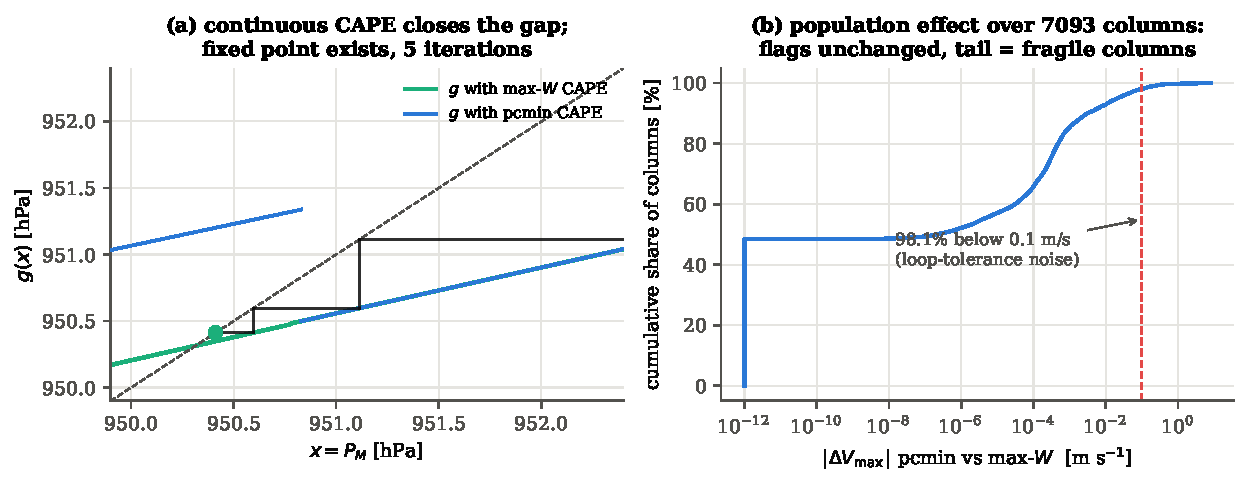
\includegraphics[width=0.98\linewidth]{fig_fix.pdf}
\caption{The repair.  (a)~On the Francine column the max-work map (teal) is
continuous through the former gap, crosses the diagonal, and the iteration
converges (dot); legacy branches (blue) shown for comparison --- away from
the gap the two maps coincide to line width.  (b)~Cumulative distribution of
$|\Delta V_{\max}|$ between conventions over the benchmark: $39\%$
bit-identical (left edge, clipped to $10^{-12}$), $98.1\%$ below $0.1\ms$,
and a $1.9\%$ tail of discontinuity-adjacent columns.}
\label{fig:fixfig}
\end{figure}

\subsection{Residual non-smoothness}\label{sec:micro}

What remains after the repair, all quantified and benign:
\begin{enumerate}
\item \emph{Newton stopping rule} in the entropy inversion (tolerance
$10^{-3}\K$): the returned temperature is a lagged iterate, so $b_j$ has
micro-jumps up to $O(10^{-3}\K)$; measured step-to-step roughness of the
repaired map is $\le7\times10^{-3}\hPa$ --- $50\times$ below the solver
tolerance, and covered by the residual check.  A literal continuity theorem
applies to the converged thermodynamic relation, not to the last bit of a
stopped Newton iterate.
\item \emph{Condensation-level formula switch} at grid nodes: same order.
\item \emph{Saturated-parcel argmax exchange} (the genuine Berge jump of
$T_O$): dormant for storm-relevant profiles (dominance margin
$\sim40\times$), but a robust API should detect ties/near-ties in the
saturated argmax and return a branch-ambiguity flag rather than silently
jumping; if it ever fires, it is physics, and residual-checked bracketing
still terminates.
\end{enumerate}

\subsection{Implementation and validation plan}

Staged so numerical and scientific changes are separable:

\begin{description}
\item[A --- diagnostics, no changed outputs.]  Expose a scalar evaluator for
$F(x)$ and CAPE diagnostics (all buoyancy roots, selected root, cumulative
work at each candidate, one-sided values); add automatic jump and
period-$k$ scans.
\item[B --- max-work kernel.]  Implement $\Emax$ in a transparent scalar
reference, then in the compiled kernel without arithmetic reassociation;
return value plus argmax metadata; classify every material difference from
legacy on the full sample before choosing the default/compatibility policy.
\item[C --- outflow semantics.]  Specify the tie rule and the relation
between the maximizing level and PI's outflow temperature; detect saturated
argmax exchanges.  If ballistic reachability is wanted for other
applications, expose it as a distinctly named free-convection diagnostic,
never as the PI default.
\item[D --- bracketed solver.]  Brent/bisection with cached CAPE
evaluations, endpoint-sign check first, distinct flags for invalid input,
entropy-solver failure, no-bracket/physical floor, and branch ambiguity;
success requires $|F(x_*)|\le\varepsilon_F$.
\end{description}

Required regression families: the exact \#77 column with one-sided values
pinned; the 1995 marginal and control pair; perturbations of SST, surface
humidity, MSL and each temperature level around both marginal cases;
analytic one-lobe/two-lobe/tangency profiles with known roots; and the full
sample with output deltas \emph{and} LNB-branch-identity changes reported.
On every successful column, verify $|F(x_*)|\le\varepsilon_F$, that the
returned CAPE equals the maximum candidate work, and that the LNB obeys the
declared tie convention.

%======================================================================
\section{Final interpretation}
%======================================================================

The causal chain, in full:
\[
\text{marginal remote buoyancy pocket}
\;\longrightarrow\; \text{hard highest-positive-node selector}
\;\longrightarrow\; \text{finite CAPE jump (helped by the clamp)}
\]
\[
\;\longrightarrow\; \text{pressure-map jump straddling the diagonal}
\;\longrightarrow\; \text{attracting, bit-exact 2-cycle}
\;\longrightarrow\; \text{``missing'' PI for a real hurricane's
counterfactual}.
\]
What is physical: multiple neutral levels, dominance exchanges between work
maxima (maximizer jumps, value continuous), and barrier transitions in the
free-convection problem.  What is conventional: calling the uppermost root
``the'' LNB.  What is artificial: letting a marginal, energetically
negligible, dynamically unreachable, effectively one-node pocket erase
$\sim224\Jkg$ of lower-tropospheric work and thereby delete the fixed point
of the pressure equation.  The repair --- maximum signed work as the CAPE
value, argmax as reported metadata, residual-checked bracketing as the
solver --- is one changed selection and one changed loop, restores an
existence proof under explicit hypotheses, and makes the two-cycle chase
disappear for the right reason.

\appendix

%======================================================================
\section{Key numbers for the failing sounding}
%======================================================================

\begin{center}
\small
\begin{tabular}{@{}ll@{}}
\toprule
quantity & value\\
\midrule
provenance & Hurricane Francine env., 18 UTC 2024-09-11, $28.6^{\circ}$N
$92.1^{\circ}$W, $\Delta\mathrm{SST}=-1.6\K$\\
SST, MSL & $28.20263672^{\circ}$C, $1014.96545\hPa$\\
levels (retained $>50\hPa$) & 37 (28)\\
cycle & $A=950.6533454438$, $B=951.2790079839\hPa$ ($B{-}A=0.6257$)\\
jump location, size & $x_d\simeq950.8289947515\hPa$, $0.837\hPa$ downward\\
one-sided residuals at $x_d$ & $+0.5073447$ / $-0.3307594\hPa$\\
slope of $g$ off the jump & $0.34$--$0.46$ (on $[946,958]$)\\
$b$ at $350\hPa$: cycle phases / at $x_d^{\mp}$ &
$+0.0137$, $-0.0350\K$ \;/\; $+7.6\times10^{-11}$, $-8.0\times10^{-11}\K$\\
$E_M$ across $x_d$ & $0 \leftrightarrow 224.23146\Jkg$ (raw signed value
$-60.9\Jkg$ before clamp)\\
$E_{MS}$, $T_O$ at $x_d$ (smooth) & $8565.00966\Jkg$, $206.1096884\K$\\
ambient CAPE $E_A$ & $1.19\Jkg$ (\#77); $0$ (both 1995 profiles)\\
corrected root (max-work, bracketed) & $x_*=950.3136889226\hPa$;
$V_{\max}=83.9065\ms$, $P_{\min}=920.7517\hPa$\\
1995 marginal: cycle / corrected root & $961.017\leftrightarrow961.671\hPa$
\;/\; $x_*=960.7687\hPa$, $V_{\max}=74.4149\ms$\\
1995 control (max-work vs legacy) & fixed point moves $0.0035\hPa$
(ballistic rule would move it $1.2\hPa$)\\
\bottomrule
\end{tabular}
\end{center}

%======================================================================
\section{Reproduction}\label{app:repro}
%======================================================================

All computations were run against branch \texttt{upstream/modernize\_eg}
(commit \texttt{abc4b4e}) of the \texttt{tcpyPI} repository, using the
committed 2024 ERA5 North-Atlantic sample and its committed outputs.  The
analysis scripts live in \texttt{discontinuity\_analysis/scripts/}:
instrumented map evaluation (\texttt{gmap.py}), fine scans
(\texttt{scan.py}), the max-work prototype and full-sample validation
(\texttt{maxw.py}, \texttt{validate.py}, \texttt{compare.py},
\texttt{dissect.py}), the survey and SST sweep (\texttt{datagen.py}), the
dominance-exchange hunt (\texttt{humphunt.py}), the reconstruction
refutation (\texttt{refine.py}), and figure generators (\texttt{plots.py},
\texttt{plots2.py}).  Every headline quantity (cycle values, jump location,
one-sided values, corrected roots, $V_{\max}$, $P_{\min}$, benchmark
statistics) was additionally reproduced by a second, independently written
implementation of the map and CAPE routines, and the two agree to the
digits shown.
The \#77 profile is the one committed in PR~\#77's failing test; the 1995
profiles are those of \texttt{tests/test\_oscillation\_rescue.py}.

\begin{thebibliography}{9}

\bibitem{bisteremanuel2002}
M. Bister and K. A. Emanuel,
``Low frequency variability of tropical cyclone potential intensity. 1.
Interannual to interdecadal variability,''
\emph{Journal of Geophysical Research}, 107(D24), 4801, 2002.
\url{https://doi.org/10.1029/2001JD000776}.

\bibitem{gilford2021}
D. M. Gilford,
``pyPI (v1.3): Tropical Cyclone Potential Intensity Calculations in Python,''
\emph{Geoscientific Model Development}, 14, 2351--2369, 2021.
\url{https://doi.org/10.5194/gmd-14-2351-2021}.

\bibitem{garner2015}
S. T. Garner,
``The Relationship between Hurricane Potential Intensity and CAPE,''
\emph{Journal of the Atmospheric Sciences}, 72, 141--163, 2015.
\url{https://doi.org/10.1175/JAS-D-14-0008.1}.

\bibitem{emanuel1994}
K. A. Emanuel, \emph{Atmospheric Convection}, Oxford University Press, 1994.

\bibitem{smith2022}
R. K. Smith,
``Effective buoyancy and CAPE: Some implications for tropical cyclones,''
\emph{Quarterly Journal of the Royal Meteorological Society}, 2022.
\url{https://doi.org/10.1002/qj.4294}.

\bibitem{pr77}
tcpyPI pull request \#77, ``Add failing test to illustrate failure of
convergence,'' including the exact regression column.
\url{https://github.com/dgilford/tcpyPI/pull/77}.

\bibitem{francine}
National Hurricane Center,
\emph{Tropical Cyclone Report: Hurricane Francine (AL062024), 9--12
September 2024}, best-track Table 1.
\url{https://www.nhc.noaa.gov/data/tcr/AL062024_Francine.pdf}.

\end{thebibliography}

\end{document}
